\subsection{Experiments}

In this section, we describe the implementation we performed for this project.
The goal was to see how the Dual Extragradient algrithm compared to the
Block-coordinate Frank-Wolfe algorithm. The task on which we performed the
evaluation was word alignment in machine translation. We extracted the dataset
from the Europarl dataset \cite{EuroparlParallelCorpus}. The data consisted of
approximately 2 million sentence pairs in both english and french. Each the
sentences in each pair were translations of one another. We extracted all
sentences and performed a clean by splitting longer sentences into shorter ones.
The goal of this step was to reduce the eventual number of matchings in
training, which could take long to solve using a LP solver. Of course, each
sentence was tokenized beforehand.

We then proceeded to implement the Dual Extragradient and BCFW algorithms using
a SVM. We had to define a feature mapping for an input sentence pair. The
features were extracted using the fastText library \cite{fastText}. This library
included a model that was previously trained to learn embeddings of words in
both english and french. We later combined the embeddings in the two languages
by applying a transformation found in \citet{chojnackiRandomGraphGenerator2010}.
This transformation consisted in applying a matrix to each vector in each
language (matrix $W$ for english and $Q$ for french). These matrices are in fact
orthogonal (i.e. $Q^T W = I$). The idea behind such a transformation is that we
sort of ``put" or ``align" both languages in the same vector space, a sort of
``middle ground". This way we can better compare the words ``cat" and ``chat" by
getting their cosine similarity measure. We combined the cosine measure of each
pair of words in the alignment by summing. The following blog post
\citet{AligningVectorRepresentations2017} provides a good intuition using maps
that are aligned.
As an example, consider the following two sentences:
\begin{itemize}
  \item This assignment was hard
  \item Ce travail etait ardu
\end{itemize}
We would compute the cosine distance for each word tuple (e.g. this/ce, this/travail,
\dots, hard/ardu). We were then able to get the highest match of each english word for
for french translation. This was how we extracted the ``labels". As the dataset was
not annotated with alignments, we had to compute those according to the procedure mentioned.

For the features, we used the concatenated embeddings of each word pairs in the
alignment. This gave us our edge score. Then, we simply performed a weighted
combination of these vectors using the edge labels as weights. To clarify what
we mean by edge labels, suppose that the edge linking ``assignment'' and
``travail'' has a value of 1. Then, we weight the vector extracted from these
two words with 1. As another example, if the edge between ``ce'' and ``ardu''
has a value of 0 (i.e. no link between the words), we do not include the vector
computed from the statistics of this word pair. This is exactly what was done in
Taskar \cite{taskarStructuredPredictionExtragradient} modulo some other
features.

\clearpage
In the implementation of BCFW, we used the solver from scipy with the simplex
method. Since the constraint matrix given by the optimization of $H_i$ in the
algorithm is unimodular, when we relax the LP, we still get a solution to the
ILP without relaxation. Thus, we take advantage of this fact and indeed use the
LP solver. The loss that we used was the $L_1$ distance between the two labels,
the proposal and the ground truth.

\subsubsection{Results}
Since running the experiments was computationally intensive and we did not
dispose of a lot of computing power, we had to restrict the training set to a
number a relatively small number of sentence pairs (100). This sanity check was
simply a hint to the general applicability of the method as we scale up the
number of training examples. We used the default $\lambda$ value of $0.01$ as
our regularizer since, we did not want to train for too many iterations before
getting decent results as per Theorem 3 found in
\citet{lacoste-julienBlockCoordinateFrankWolfeOptimization2013}. We were able to
get the following results for the BCFW algorithm:


To further motivate our intuition and to make sure the algorith ran properly, we
used the local scene dataset \cite{JMLR:v15:mueller14a} from PyStruct to train a
SVM using BCFW. It consisted of vectors of size 294 for the features of each
training example (images). Each image was labeld according to the type of
objects that were present in the scene.\\
These were:
\begin{equation}
  beach \quad\cdot\quad sunset \quad\cdot\quad fall \quad\cdot\quad foilage \quad\cdot\quad field
  \quad\cdot\quad mountain  \quad\cdot\quad urban
\end{equation}

These 6 classes were not mutually exclusive so we had a total of $2^6=64$
possible labels. Training using all possible edges allowed to fully capture the
complex relationships between them. The duality gap on the training data is
given by the figure \ref{fig:bcfwLoss}.

For the dual extragradient, we were only able to run the algorithm on a dataset
of images \citet{vemulapalliCompactEmbeddingFacial2018}. These were tuples of 3 images and a person
hand-picked two images in each 3-tuple that resembled each other the most. Using the
extragradient algorithm, we were able to get convergence but the results were not 
satisfying. We only obtained 46\% accuracy on the prediction, which would compare 
with 33\% if we had a random predictor (3 choose 2 gives 3  possibilites hence 33\%).
Thus, it motivated our change of dataset to obtain better results. We also moved on to
the BCFW algorithm as we had not implemented it yet.

\begin{figure}[htbp!]
  \center
  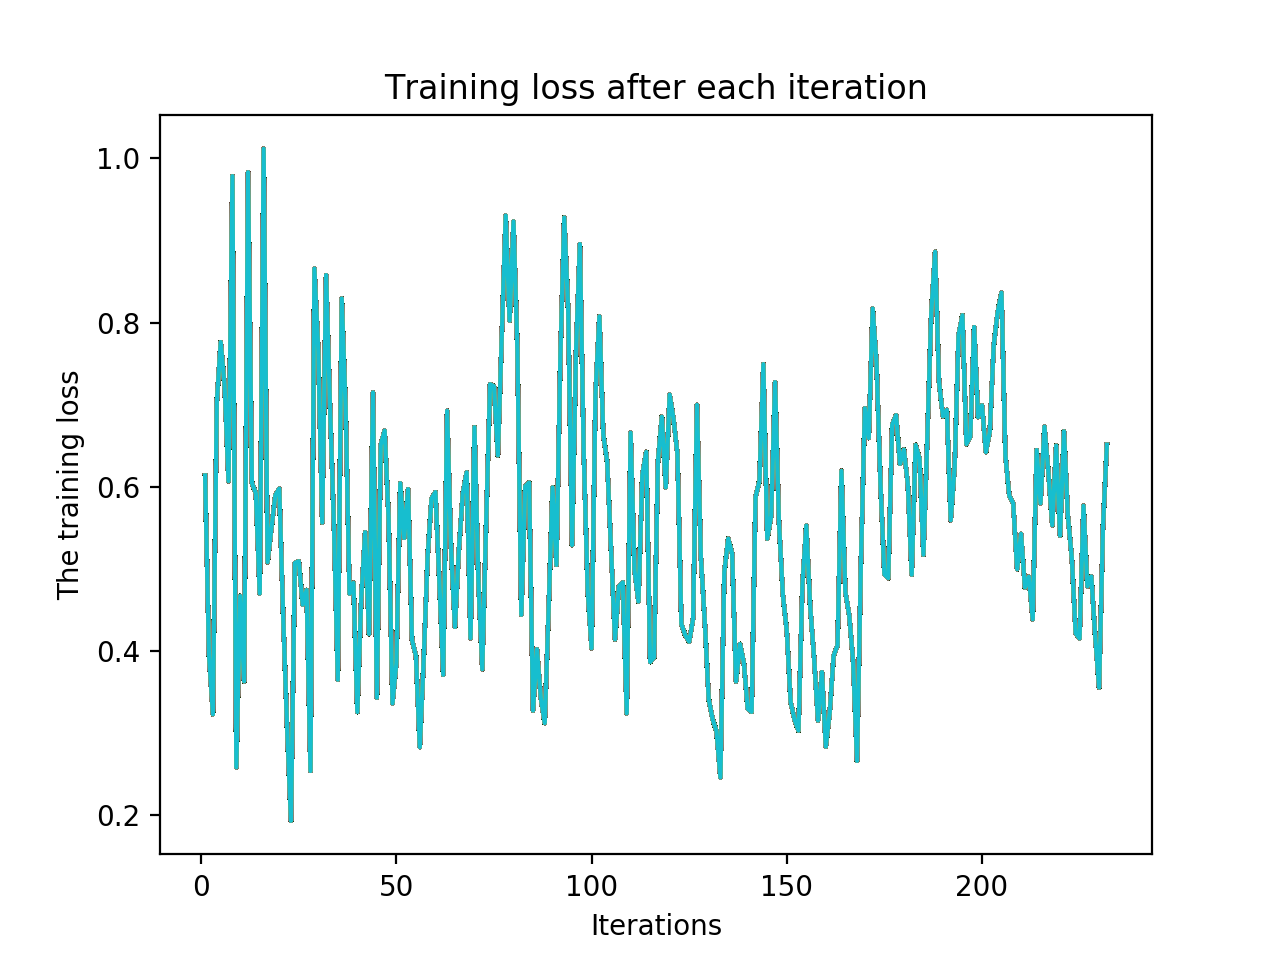
\includegraphics[width=0.8\textwidth]{loss_bcfw.png}
  \caption{BCFW loss}
  \label{fig:bcfwLoss}
\end{figure} 
\begin{figure}[htbp!]
  \center
  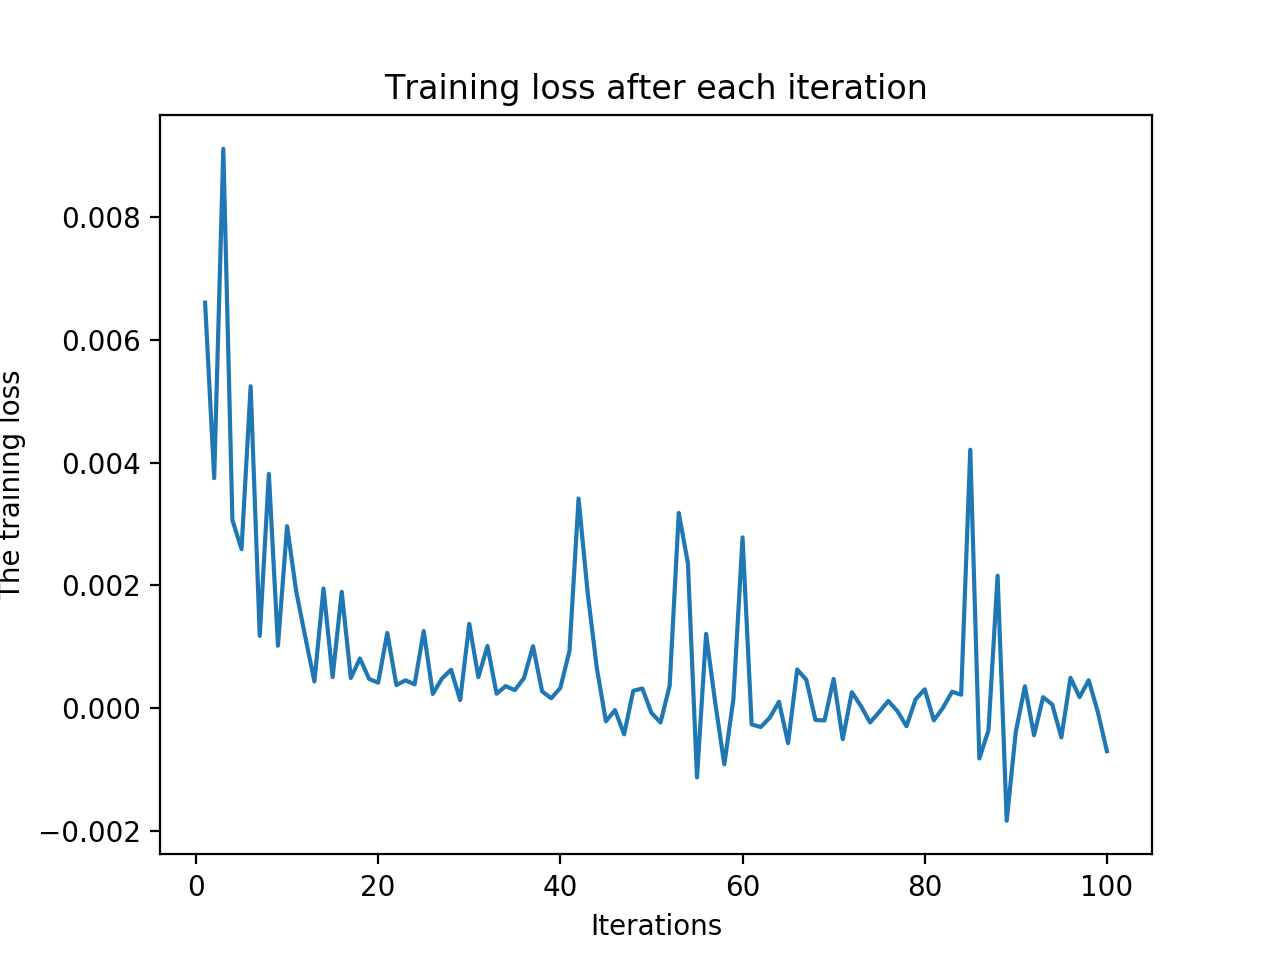
\includegraphics[width=0.8\textwidth]{pystruct_scene.png}
  \caption{pystruct scene}
  \label{fig:pystruct}
\end{figure} 

%FEC : vemulapalliCompactEmbeddingFacial2018,
%fest :mikolovAdvancesPreTrainingDistributed2017,
%pystryct: JMLR

%%% Local Variables:
%%% mode: latex
%%% TeX-master: "mainProject"
%%% End:
